\documentclass{homework}

\title{Homework template}
\author{Christoffer Corfield Aakre}
\date{
}

\begin{document}

\newcommand{\fe}{F_{\text{engine}}}

\maketitle

\part


\exercise

Let $\vec{N}$, $m\vec{g}$ and $\vec{f}$ be the normal force, weight of the block, and the frictional force, respectively. Let us choose Cartesian axes such that $\hat{x}$ points down the inclined plane,
and $\hat{y}$ points up perpendicularly from the plane. See the below diagram:
\begin{figure}
    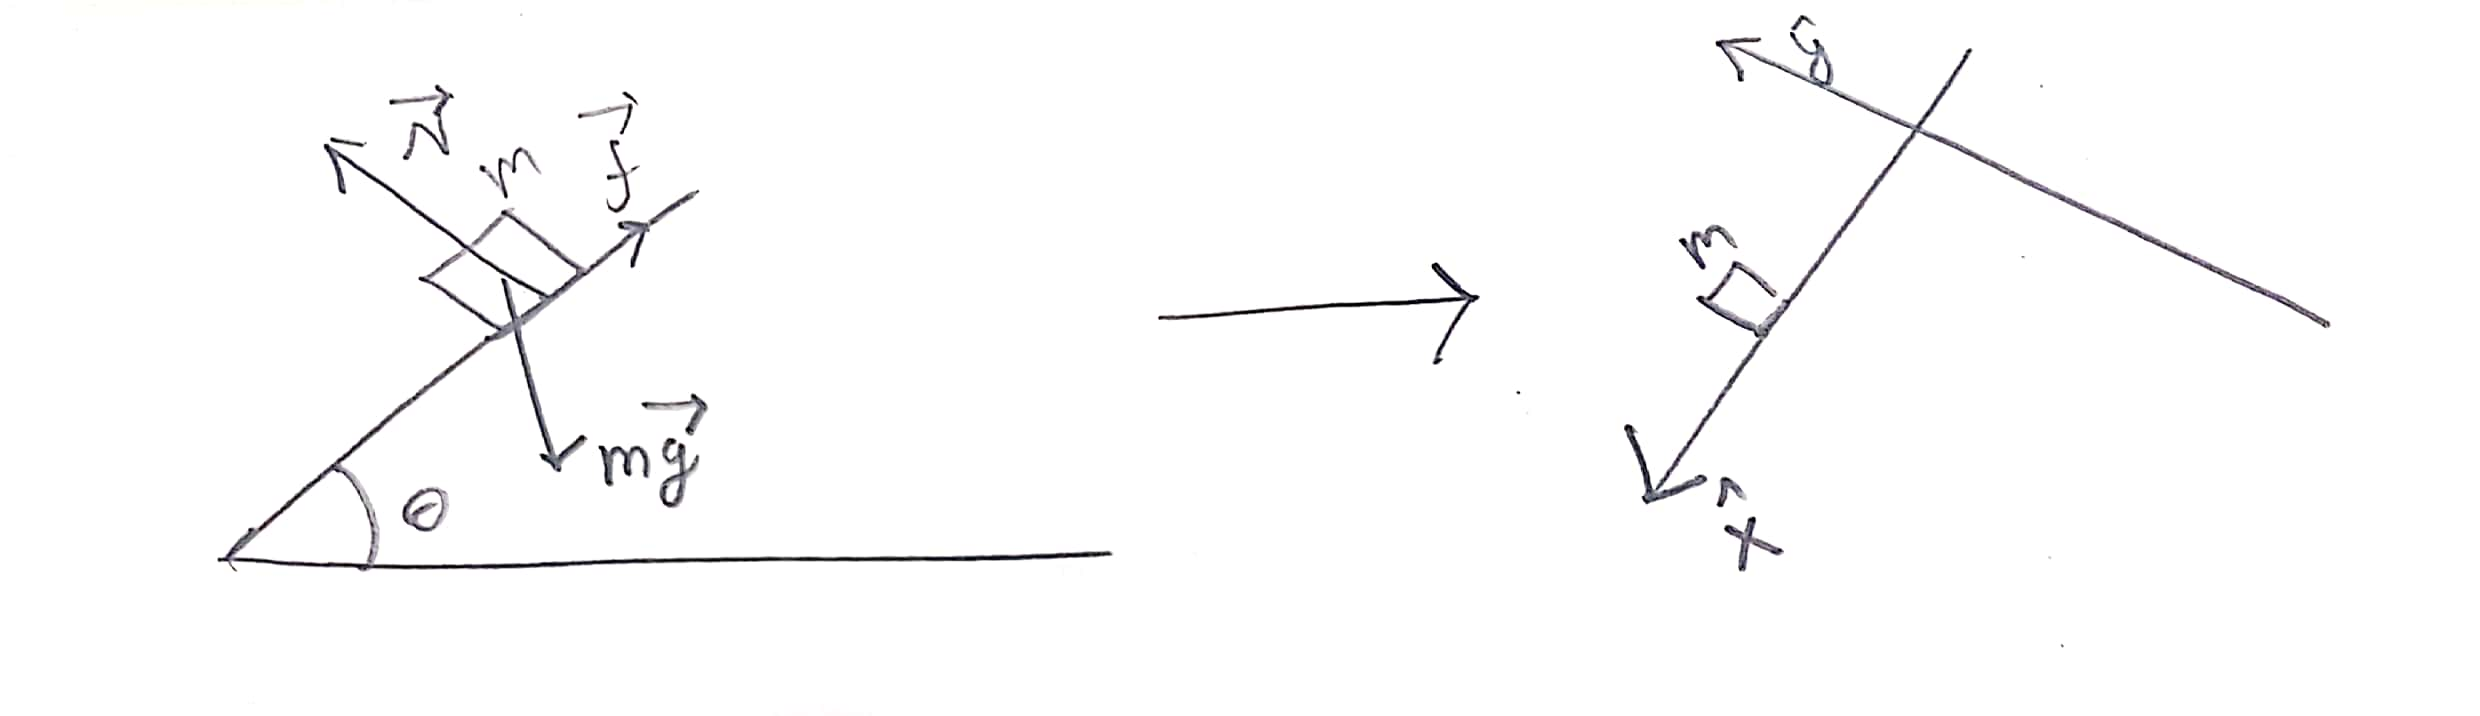
\includegraphics{inclined-plane}
\end{figure}

Then, $\vec{N}$ points only in the $y$ direction, and $\vec{f}$ points only in the $x$ direction. Now we look at $m\vec{g}$.
See the below diagram:

\begin{figure}
    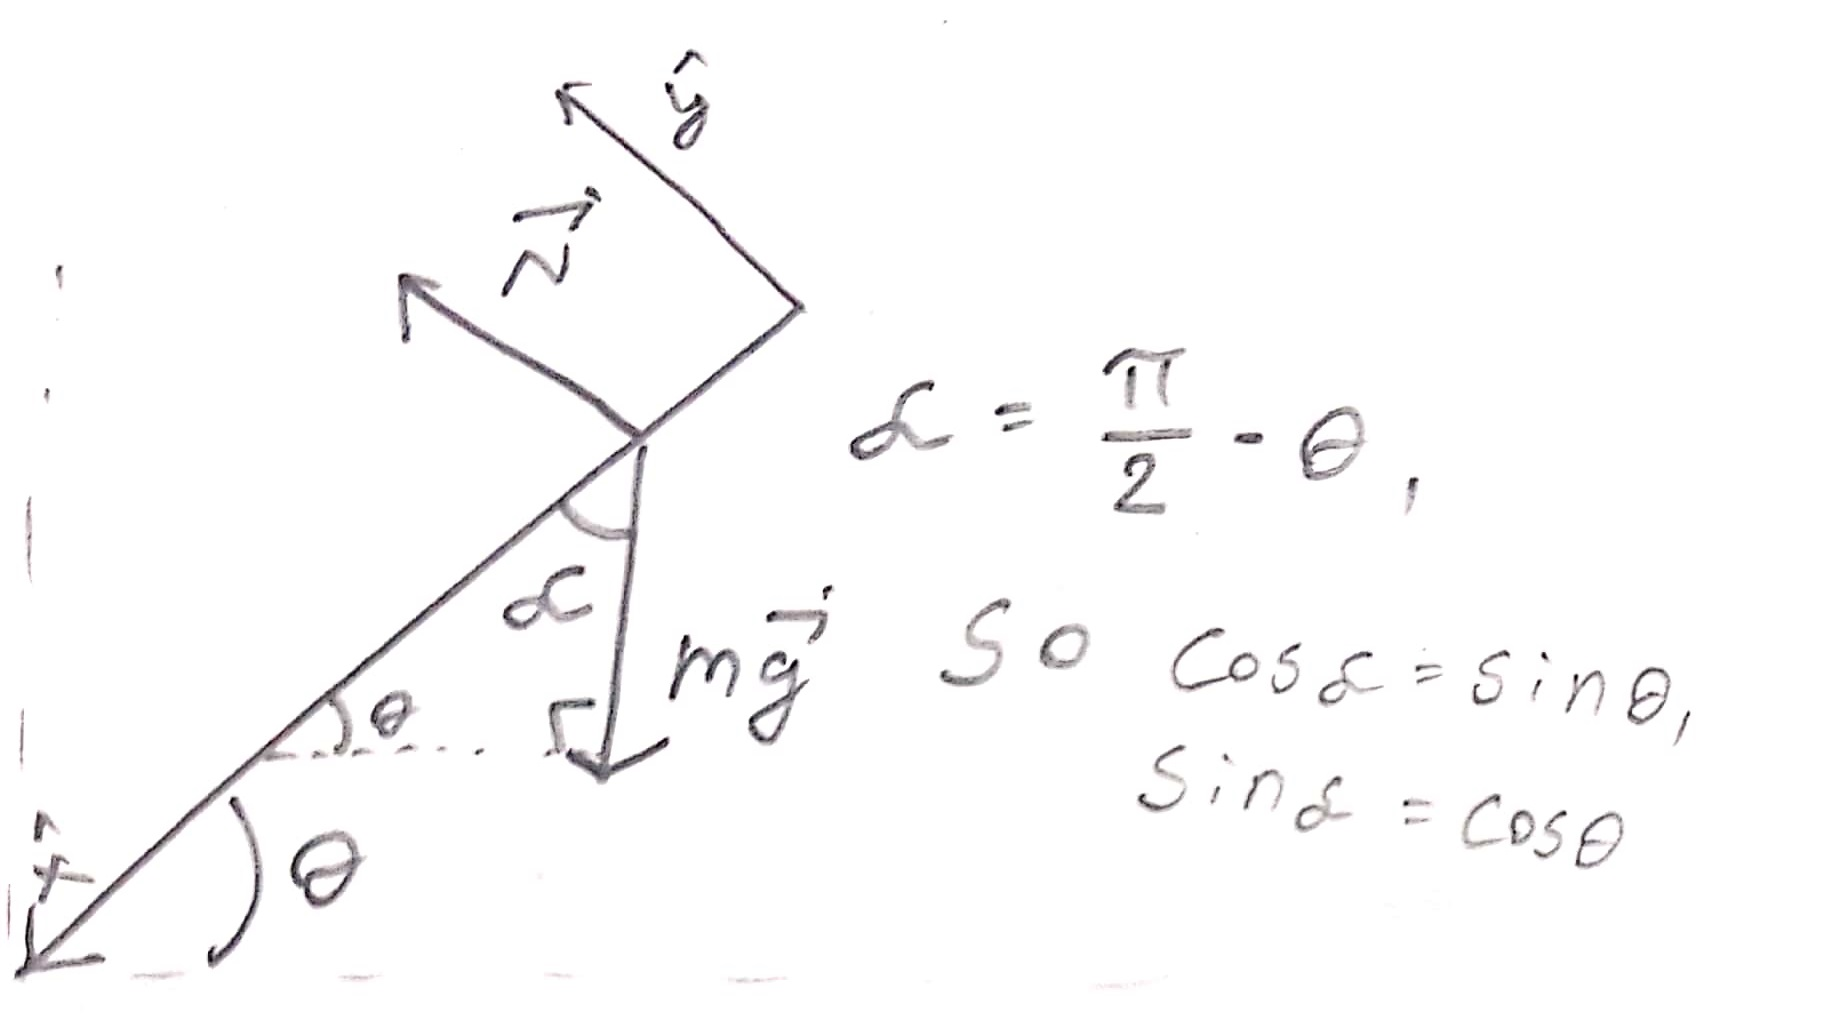
\includegraphics{diagram2}
\end{figure}

So, since $\lvert m\vec{g} \rvert = mg$, we have
\begin{equation*}
    m\vec{g} = mg\sin\theta \hat{x} - mg\cos\theta \hat{y}    
\end{equation*}

Since the net force is $0$, we then have
\begin{align*}
    m\vec{g} &= mg\sin\theta \hat{x} - mg\cos\theta \hat{y}, \\
    \vec{N} &= mg\cos\theta \hat{y}, \\
    \vec{f} &= -mg\sin\theta \hat{x}
\end{align*}

Plugging in $m = \SI{0.1}{\kilo\gram}$, $g = \SI{10}{\meter\per\second\squared}$, $\theta = \SI{45}{\degree}$, we have

\begin{align*}
    m\vec{g} &= \frac{\sqrt{2}}{2}\hat{x} - \frac{\sqrt{2}}{2}\hat{y}, \\
    \vec{N} &= \frac{\sqrt{2}}{2}\hat{y}, \\
    \vec{f} &= -\frac{\sqrt{2}}{2}\vec{x} .\\
\end{align*}



\exercise
The acceleration $a(t)$ is given by 

\begin{equation*}
    a(t) = Ae^{=kt}.
\end{equation*}

Since the car starts from rest, at time $t$, its speed $v(t)$ will be given by
\begin{align*}
    v(t) &= \int_0^t a(t) \mathop{dt} \\
    &= \int_0^t Ae^{-kt} \mathop{dt} = -\frac{A}{k} \int_0^{-kt} e^u \mathop{du} \\
    &= -\frac{A}{k}e^u \big\rvert_0^{-kt} = -\frac{A}{k}(e^{-kt} - e^0) \\
    &= \frac{A - Ae^{-kt}}{k}. \\
\end{align*}

The distance travelled from time $0$ to time $t$ is given by

\begin{align*}
    x(t) &= \int_0^t v(t) \mathop{dt} \\
    &= \int_0^t \frac{A - Ae^{-kt}}{k} \mathop{dt} = \frac{A}{k} \int_0^t (1 - e^{-kt}) \mathop{dt} \\
    &= \frac{At}{k} - \frac{A}{k}\int_0^t e^{-kt} \mathop{dt} = \frac{At}{k} = \frac{A}{k^2} \int_0^{-kt} e^u \mathop{du} \\
    &= \frac{At}{k} + \frac{A}{k^2} e^u \big\rvert_0^{-kt} = \frac{At}{k} + \frac{A}{k^2}(e^{-kt} - 1) \\
    &= \frac{A}{k^2} (kt + e^{-kt} - 1). \\
\end{align*}

Now, the net force $F$ on the engine is given by

\begin{equation*}
    F = F_{\text{engine}} - cv
\end{equation*}

Rewriting this as a differential equation, we have

\begin{equation*}
    m\frac{dv}{dt} = \fe - cv.
\end{equation*}

Separating variables and integrating, then solving for $v$ yields the following:

\begin{align*}
    \int_0^v \frac{m}{\fe - cv} \mathop{dv} = \int_0^t \mathop{dt} \\
    t = -\frac{m}{c}\ln\left(\frac{\fe - cv}{\fe}\right) \\
    -\frac{ct}{m} = \ln\left(\frac{\fe - cv}{\fe}\right) \\
    e^{-ct / m} = \frac{\fe - cv}{\fe} \\
    \fe - cv = \fe e^{-ct / m} \\
    cv = \fe - \fe e^{-ct / m} \\
    v = \frac{\fe}{c} (1 - e^{-ct / m}) \\
\end{align*}

The final speed $v_f$ is given by

\begin{align*}
    v_f &= \lim_{t \to \infty} v(t) \\
    &= \lim_{t \to \infty} \frac{\fe}{c} (1 - \cancelto{0}{e^{-ct / m}}) \\
    &= \frac{\fe}{c}
\end{align*}

Another, perhaps easier to calculate the final speed would be to notice that at
the final speed, the net force will be zero, so

\begin{equation*}
    \fe = cv_f \implies v_f = \frac{\fe}{c}
\end{equation*}

but solving the differential equation is more straightforward, and also leads to a velocity function.

\exercise
The kinetic energy of a mass $M$ travelling at a speed $v$ is given by

\begin{equation*}
    E_k = \frac{1}{2}Mv^2.
\end{equation*}

\begin{proof}
Let us start by defining Kinetic Energy. If we send a ball with mass $M$ rolling with speed $v$ (Assuming no friction etc.), then it will have some kinetic energy. If the ball collides with a wall and stops completely, then the ball will release energy in the form of heat, sound, etc. The sum of all the released energies is the kinetic energy that the ball \textit{had} before colliding. We assume that the Kinetic energy $E(m, v)$ only depends on the mass and the speed.

If we have a ball with mass $2M$ and speed $v$, then just before the ball collides with a wall, we can slice it in half, and we will have two balls with mass $M$, still travelling at speed $v$. We would expect the balls to still release the same amount of energy during the collision with the wall, so 

\begin{equation*}
    E(2M, v) = 2E(M, v)
\end{equation*}

Now we will consider the effect of the speed. Consider two balls of mass $M$ travelling towards each other at speed $v$. See the below diagram:

\begin{figure}
    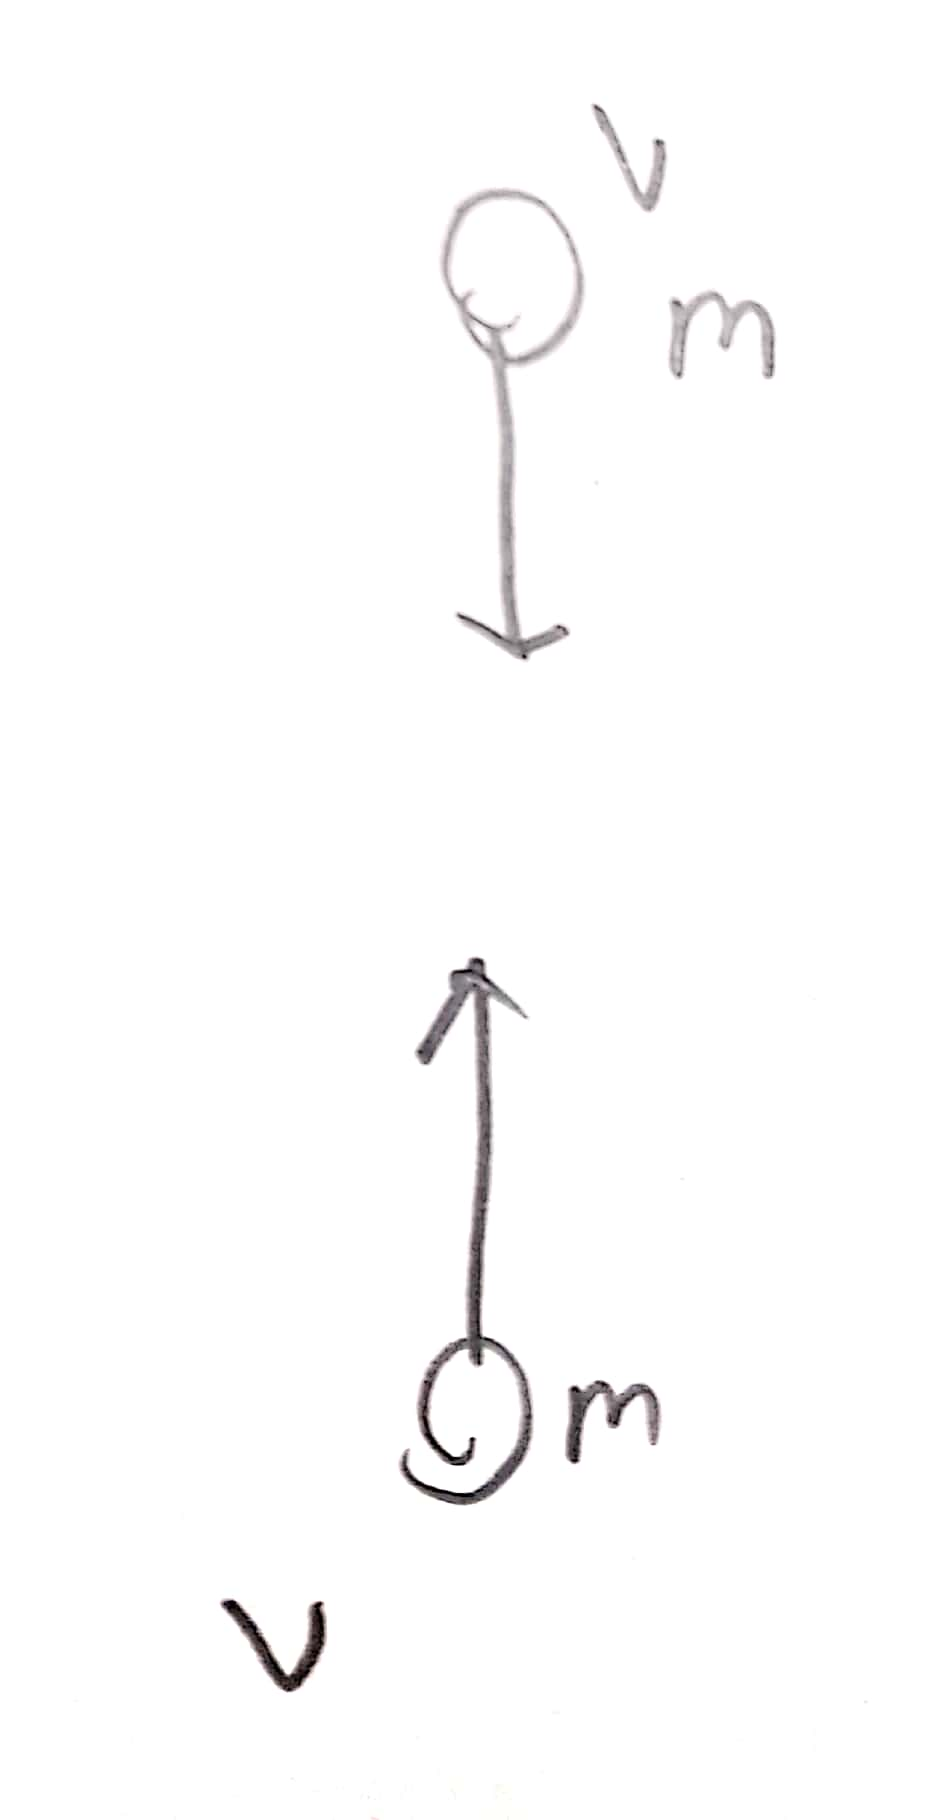
\includegraphics{towards}
\end{figure}

The balls collide, and both stop completely. Thus, the energy $\Delta E$ released is given by 

\begin{equation*}
    \Delta E = E(M, 2v).
\end{equation*}

Now imagine the balls are on a train that is moving at a speed $v$ as the same direction as one of the balls, and consider the reference frame of an observer outside the train watching the train move. Even though the velocities are now different, the energy released must still be the same in this reference frame. In this reference frame, one ball is moving at a speed $2v$ and the other ball is standing still. See the below diagram:

\begin{figure}
    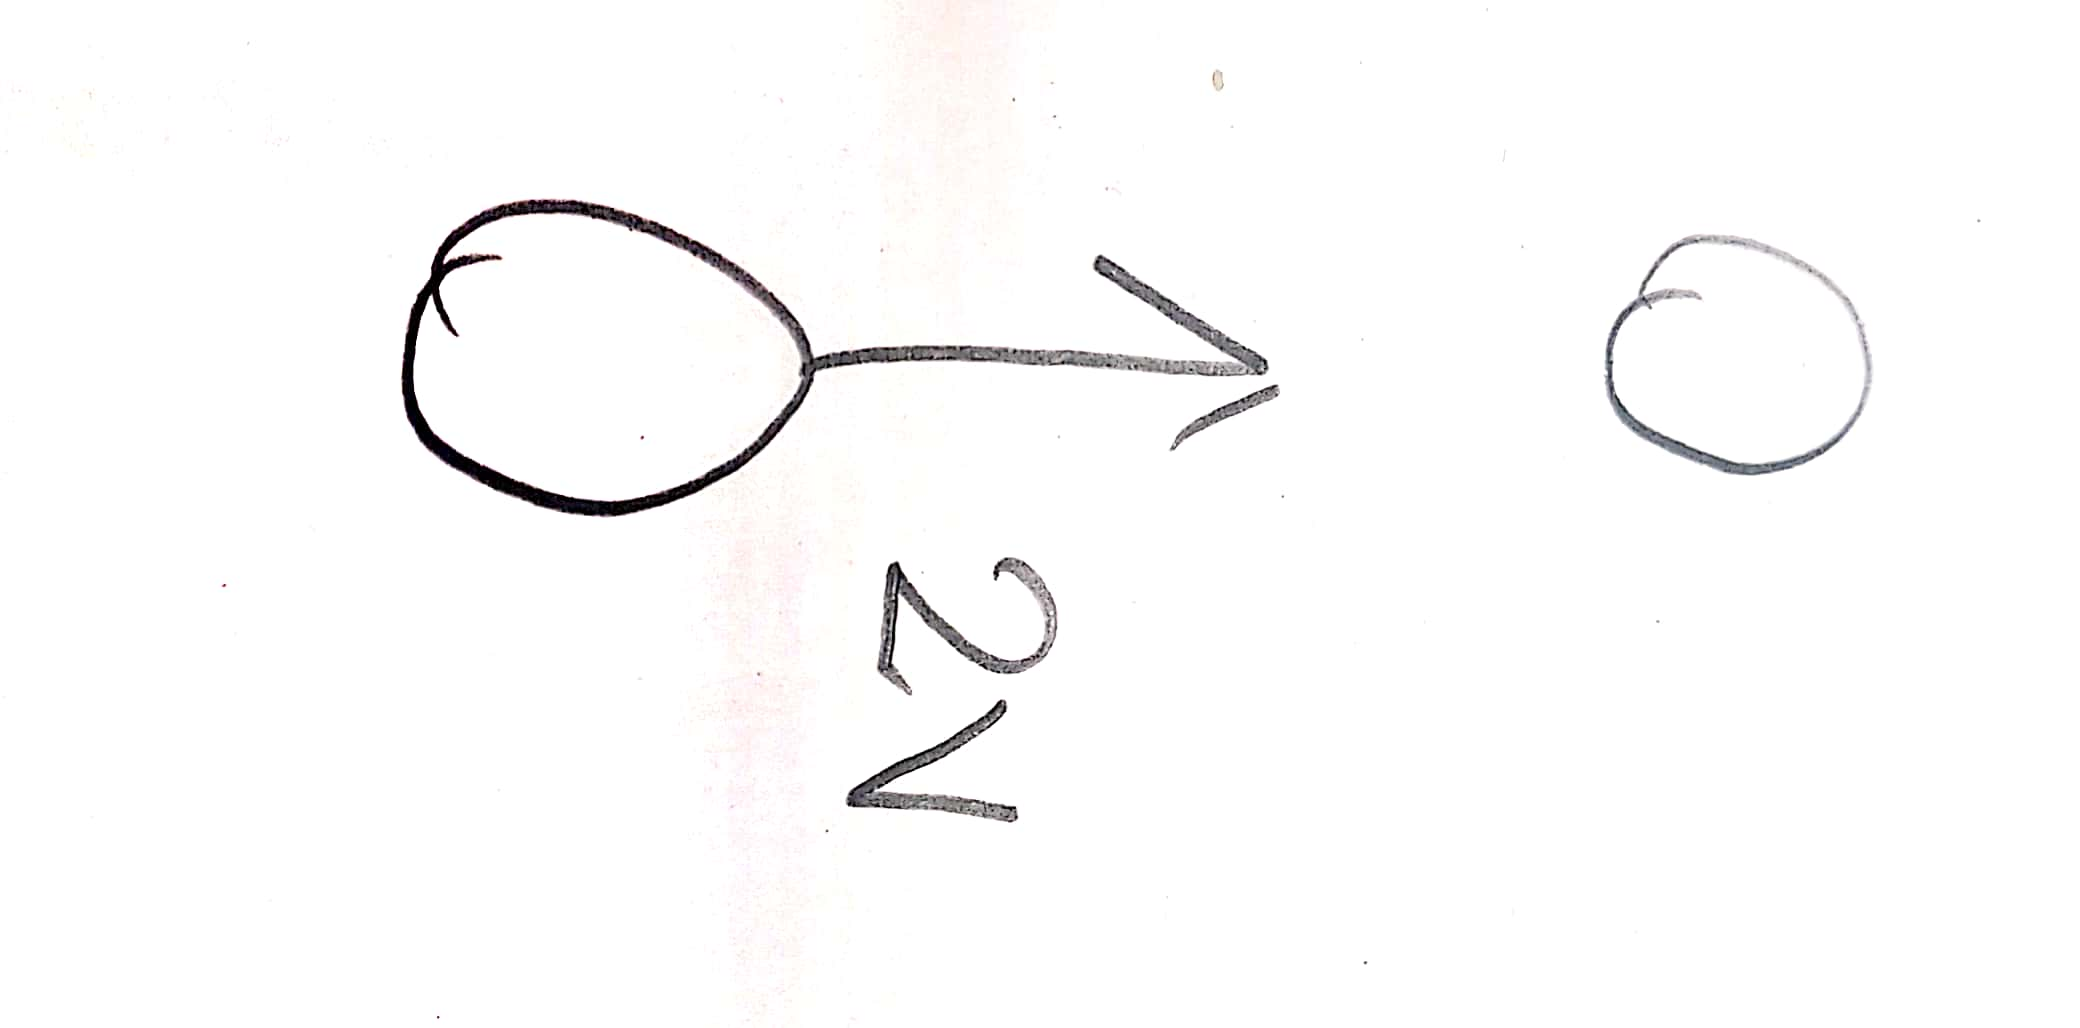
\includegraphics{2v}
\end{figure}

After the colission, the balls are both moving together at a speed $v$. So, in this reference frame, the energy released is

\begin{equation*}
    \Delta E = E(2M, v) - 2E(M, v).
\end{equation*}

$\Delta E$ must be the same in both reference frames, so we have

\begin{equation*}
    E(M, 2v) - 2E(M, v) = 2E(M, v) \implies E(M, 2v) = 4E(M, v).
\end{equation*}

This implies that $E$ is quadratic in $v$, and we can go further and have balls moving at speeds $nv$ rather than $2v$, and come to the same conclusion. So, now we have

\begin{equation*}
    E(M, v) = kmv^2 \text{ for some $k\in\mathbb{R^+}$}.
\end{equation*}

We can set $k$ to any number we like, and then derive the formula for work, and hence the other energy formulas, and we see that if we let $k = \frac{1}{2}$, then we can write a lot of energy formulas without a constant, e.g. $E = mgh$, $W = \int \vec{F} \cdot \mathop{d\vec{r}}$, etc., so we let $k = \frac{1}{2}$, and so we have

\begin{equation*}
    E_k = \frac{1}{2}mv^2.
\end{equation*}
\end{proof}
From the kinetic energy formula we can now derive the work force relation, and other formulas, in contrast to starting by assuming $W = \int \vec{F} \cdot \mathop{d\vec{r}}$. I think this derivation is more intuitive.

The potential energy $E_p$ of a spring with spring constant $k$ displaced from its equlibrium by $x$ is given by

\begin{equation*}
    E_p = \frac{1}{2}kx^2.
\end{equation*}
\begin{proof}
The restoring force (in one dimension, so we work with scalars), $F$ on a spring with spring constant $k$ that has been displaced from its equilibrium position by $x$ is given by

\begin{equation*}
    F = -kx.
\end{equation*}

The potential energy $E_p$ in the spring is equal to the work done against the restoring force, so we have

\begin{align*}
    E_p &= -W = -\int_0^x F \mathop{dx} \\
    &= \int_0^x kx \mathop{dx} \\
    &= \frac{1}{2}kx^2\big\rvert_0^x \\
    &= \frac{1}{2}kx^2.
\end{align*}
\end{proof}
Assuming there is no energy loss due to external forces, all the potential energy will be converted to kinetic energy, so we have

\begin{align*}
    &\cancel{\frac{1}{2}}Mv^2 = \cancel{\frac{1}{2}}kx^2 \\
    &v^2 = \frac{k}{M}x^2 \\
    v &= \sqrt{\frac{k}{M}x^2} \\
    &= \sqrt{\frac{k}{M}}x.
\end{align*}

\exercise

To keep the mass moving along the circular path, the spring must provide a centripetal force $\vec{F}$ given by

\begin{equation*}
    \vec{F} = -Mr\omega^2 \hat{r},
\end{equation*}

assuming that we are working in polar coordinates.

This must equal the inwards radial force from the spring, which is given by

\begin{equation*}
    -kx\vec{r}.
\end{equation*}

So, we have

\begin{align*}
    \cancel{-\vec{r}} \times kx = -\vec{r} \times \cancel{Mr\omega^2}  \\
    kx = Mr\omega^2 \\
    k = \frac{Mr\omega^2}{x}
\end{align*}

Since $r$ is the radius of the circular motion, $d$ d is the natural length of the spring,
and $x$ is the extension beyond $d$ of the spring, then 

\begin{equation*}
    x + d = r \implies x = r - d.
\end{equation*}

So,

\begin{equation*}
    k = \frac{Mr\omega^2}{r - d}.
\end{equation*}

\exercise

(Working in polar coordinates)
For reference,

\begin{align*}
    x &= r\cos\theta, \\
    y &= r\sin\theta, \\
    r &= \sqrt{x^2 + y^2}, \\
    \theta &= \arctan\left(\frac{y}{x}\right), \\
    \hat{r} &= \cos\theta \hat{x} = \sin\theta \hat{y}, \\
    \hat{\theta} &= -\sin\theta \hat{x} = \cos\theta \hat{y},
\end{align*}

and so

\begin{align*}
    \mathop{d\hat{r} / dr} &= 0, \\
    \mathop{d\hat{\theta} / dr} &= 0, \\
    \mathop{d\hat{r} / d\theta} &= \hat{\theta}, \\
    \mathop{d\hat{\theta} / d\theta} &= -\hat{r}. \\
\end{align*}

In polar coordinates, the acceleration vector $\vec{a}$ is given by

\begin{equation*}
    \vec{a} = \hat{r}(\ddot{r} - r\dot{\theta}^2) + \hat{\theta}(r\ddot{\theta} + 2\dot{r}\dot{\theta}).
\end{equation*}

\begin{proof}
\begin{align*}
    &\vec{r} = r\hat{r} \\
    \vec{v} &= \mathop{\frac{d\vec{v}}{dt}} \\
    &= \mathop{\frac{d}{dt}}(r\hat{r}) \\
    &= \dot{r}\hat{r} + r\dot{\hat{r}} \\
    &= \dot{r} + r \mathop{\frac{d\hat{r}}{d\theta}} \mathop{\frac{d\theta}{dt}} \\
    &= \dot{r}\hat{r} - r\dot{\theta}\hat{\theta} \\
    &\vec{a}= \mathop{\frac{d\vec{v}}{dt}} \\
    &= \mathop{\frac{d}{dt}}(\dot{r}\hat{r} - r\dot{\theta}\hat{\theta}) \\
    &= \ddot{r}\hat{r} + \dot{r}\dot{\hat{r}} + \dot{r}\dot{\theta}\hat{\theta} + r\ddot{\theta}\hat{\theta} + r\dot{\theta}\dot{\hat{\theta}} \\
    &= \ddot{r}\hat{r} + 2\dot{r}\dot{\theta}\hat{\theta} + r\ddot{\theta}\hat{\theta} - r\dot{\theta}^2 \hat{r} \\
    &= \hat{r}(\ddot{r} - r\dot{\theta}^2) + \hat{\theta}(r\ddot{\theta} + 2\dot{r}\dot{\theta}) \\
\end{align*}
\end{proof}
For the snowball given in the exercise, we have 

\begin{align*}
    \ddot{r} &= 0, \\
    \dot{r} &= \SI{-20}{\meter\per\second}, \\
    r &= (3 - 20t)\SI{}{\meter}, \\
    \ddot{\theta} &= 0, \\
    \dot{\theta} &= \SI{3.33}{\per\second} \\
\end{align*}

Plugging in these values gives

\begin{equation*}
    \vec{a} = \hat{r} \times (222.2t - 33.3)\SI{}{\meter\per\second\squared} - \hat{\theta} \times \SI{133.33}{\meter\per\second\squared}
\end{equation*}

\pagebreak

\part
\exercise
\exercisepart hey
\begin{subexercises}
    \item hey
    \item bye
\end{subexercises}

\exercisepart

\begin{subexercises}
    \item lol
\end{subexercises}

\exercisepart so we do this, and then the following
\exercisepart yep

\question{Question 1}
\exercisepart hey
\exercisepart another one
\begin{subexercises}
    \item the first one
    \item second
    \item you guessed, it number three!
\end{subexercises}

\end{document}
